\section{State of the Art} \label{sec:sota}
This section will discuss the existing smart materials that are currently studied and used in the domain of actuators. The different techniques and integration systems will also be presented with the goal to compare the various approaches currently used.

\subsection{Smart materials} \label{subsec:Smartmaterials}
In the field of engineering, ranging from haptics, automation and bio-medical fields, there has been a need  to create actuators that are lightweight, compact and having force output. This creates a need for materials that can deliver high forces and strokes while remaining light and small meaning that the materials need to have a high work output.

On the basis of creating an actuator that can meet the demands of the currently implemented strategies while at the same time pushing the limits of the current technology, a thorough investigation of the available smart materials must be conducted. These materials have the ability to react mechanically to an external stimulus such as thermal electrical or magnetic and are thus referred to as \emph{smart} or \emph{active materials}. There exist numerous types of smart materials and based on their properties, they can be classified into many types based on their activation methods\cite{damodharan_review_2018}.
% \begin{itemize}
% 	\item Piezoelectric materials
% 	\item Magneto-strictive materials
% 	\item Electro-active polymers
% 	\item Shape Memory Alloys
% \end{itemize}

The aim of this project is to adapt the various smart materials to harness their specific behaviour and fabricate smart actuators. This implies that the system that incorporates the material is equally critical for the conception of the actuator. This section of the report will delved into different strategies used to harness the specific behaviours of the smart materials and integrate them into actuators.

\subsubsection{Piezoelectric Materials}
Piezoelectric (PZT) materials are a well known type of smart material that reacts to voltages. These materials are already commercially available in various different gripper systems. The company PI\cite{noauthor_p-604_2018} is a supplier of PZT actuators and many more such suppliers already exist.

\begin{wrapfigure}{r}{0.45\textwidth}
	\centering
	% \vspace{-10pt}
	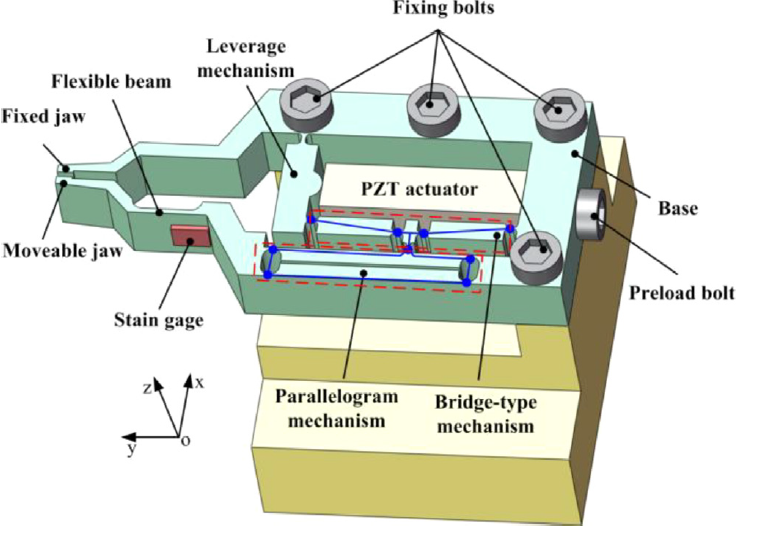
\includegraphics[width=0.4\textwidth]{Figures/PZT_grip.png}
	\caption{Mechanism of the PZT gripper\cite{liang_design_2018}.}
	% \vspace{-15pt}
	\label{fig:PZT_grip}
\end{wrapfigure}

PZT actuators are widely used due to the fact that they have small volumes, high output force ($\sim10^5$ J/m$^3$) and fast response times (10$^6$ Hz)\cite{faran_ferromagnetic_2016}. But generally these materials have quite a small maximum stroke, generally around 20 \micrometer for a 0.5 mm stack\cite{rupitsch_piezoelectric_2019}. This implies that PZT actuators will require the integration of amplifiers that will increase the total displacement of the actuator. The work performed by Liang et al., 2018\cite{liang_design_2018} displays a micro-gripper that is comprised of a PZT along with an integrated amplifying system. The study uses flexure-based mechanical structures as an amplifier so as to create a high stroke gripper without a great increase in the total volume of the gripper.

An interested approach to designing the amplification system has been observed in the study performed by Ruiz and Sigmund, 2018\cite{ruiz_optimal_2018}. In this work, a large displacement PZT microgripper was designed from a rectangular plate using topology optimization. Here, the PZT plate is sandwiched between two electrodes and an input voltage is applied. This voltage will generate an electric field and will create a deformation in the PZT structure. The optimisation strategy is to increase the deformation by varying the shape and dimensions of the total structure. This strategy could be used in not just this instance but to optimize the actuation of any actuator built around an active smart material.

Based on the literature and the specifications of the gripper, the volume of the piezoeletric material can be calculated to be 150 mm$^3$.

\subsubsection{Electro-Active polymers}
Electroactive Polymers (EAP) have the ability to alter their mechanical behaviour such as a change in shape or size when exposed to an electric field. EAPs emerged in the last few decades exhibiting large strains when exposed to electrical stimulus \cite{bar-cohen_artificial_2005}.

EAP can generate high strains, with Dielectric elastomers (DE) such as silicone exhibiting strains of about 63\%\cite{kornbluh_electroactive_2004}. EAP materials can also exhibit greater response times, in the order of 10$^5$ Hz, when compared to smart materials such as shape memory alloys, which will be explored in the next section. EAP can be very useful for their fast actuation times, low density and greater resilience and can, thus, be very convenient when create mechanical devices that are light weight and compact.
% Dielectric Electroactive Polymers (DEAP) are based on the electromechanical behaviour of dielectric films when a compliant electrode is placed on each surface and a voltage is applied across them. This results in the DEAP to shrink in thickness and expand in area.
%
% \begin{figure}[H]
%     \centering
%     \begin{subfigure}[t]{0.45\textwidth}
% 			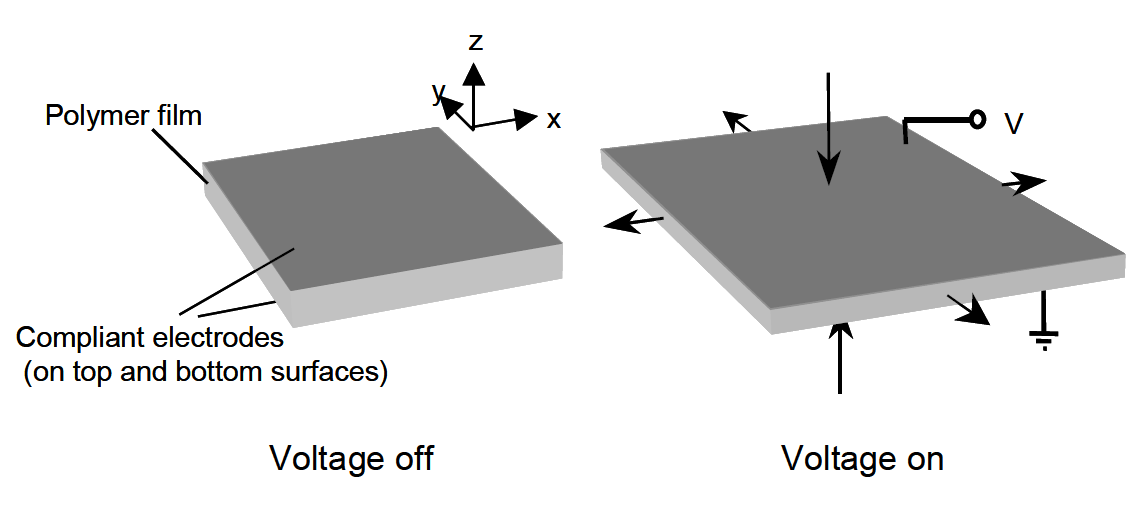
\includegraphics[width=\textwidth]{Figures/DEAP_fig.png}
% 			\caption{Functional element of dielectric elastomer actuators. Polymer film compresses in thickness and expands in area when a voltage is applied across the film.}
% 			\label{fig:DEAP_fig}
%     \end{subfigure}
%     ~ %add desired spacing between images, e. g. ~, \quad, \qquad, \hfill etc.
%       %(or a blank line to force the subfigure onto a new line)
%     \begin{subfigure}[t]{0.45\textwidth}
% 			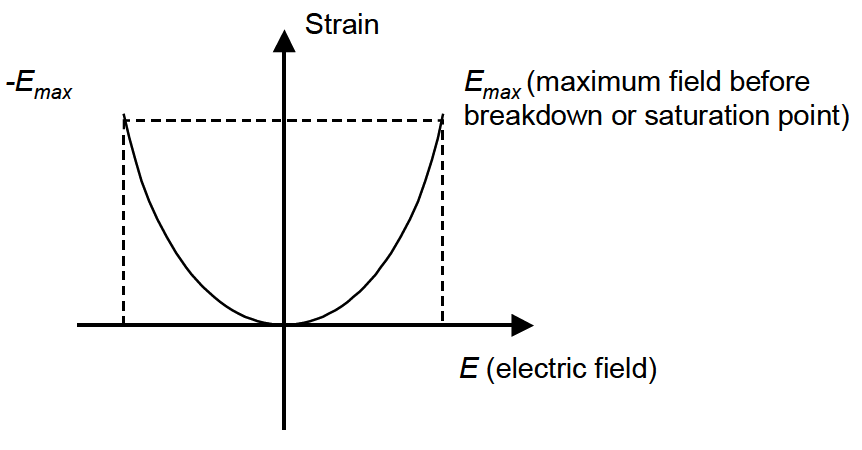
\includegraphics[width=\textwidth]{Figures/DEAP_curve.png}
% 			\caption{Typical thickness or planar strain response to applied electric field for a film with no external loads.}
% 			\label{fig:DEAP_curve}
%     \end{subfigure}
% 		\caption{Principle of operation of dielectric elastomer actuators\cite{kornbluh_electroelastomers:_2002}.}
% 		\label{fig:DEAP}
% \end{figure}

The behaviour of the film is caused by the interaction of the electrostatic charges that are created on the opposing electrodes. By applying a voltage on the two electrodes, the electrodes are subjected to opposite charges cause an attractive force between them. The pressure, $p$, created can be calculated\cite{thummala_analysis_2012} using the following relationship :
\begin{equation}
	\label{eq:DEAP_p}
	p = \varepsilon_r\varepsilon_0E^2 = \varepsilon_r\varepsilon_0(V/t)^2
\end{equation}
where $\varepsilon_r$ and $\varepsilon_0$ are the permittivity of free space and the relative permittivity of the polymer respectively, $E$ is the electric field, $V$ is the voltage applied across the electrodes and $t$ is the thickness of the dielectric material.

\begin{wrapfigure}{l}{0.45\textwidth}
	\centering
	% \vspace{20pt}
	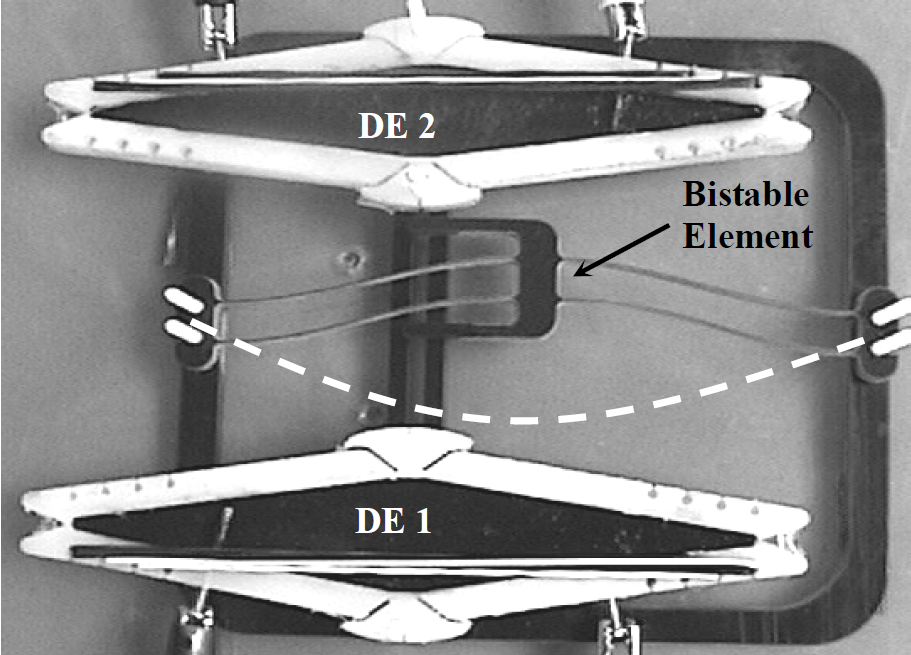
\includegraphics[width=0.4\textwidth]{Figures/DEAP_flipflop.png}
	\caption{Flip-flop bistable actuator concept\cite{plante_compliant_2005}.}
	% \vspace{-15pt}
	\label{fig:DEAP_flipflop}
\end{wrapfigure}
\paragraph{Dielectric elastomer} (DE) actuators are comprised of an elastomeric film that is platted on both sides with a compliant electrode as shown in figure.The system is actuated when a high voltage is applied between the two electrodes.The main drawback of using DE actuators are the fact that they have very small fatigue life which is around $10^3$ cycles\cite{chen_preliminary_2017}. By attempting to use the DE actuators in a continuous fashion, it will result in a short lifetimes and low reliability. In the paper written by Plante et al,. 2005\cite{plante_properties_2007,chouinard_bistable_2012} or by Wang et al., 2018\cite{wang_design_2018}, the teams overcome the burdens of short fatigue life by coupling the DE actuator with a bistable element. Here, the work displays DE actuators and a flip-flop bistable mechanism, where two agonistic-antagonistic actuators move a buckled beam back and forth. The DE actuator works as an external trigger mechanism that, when actuated, will force the bistable element into its opposing stable state.

The work shows that the approach to use an antagonistic actuators with a smart material as a trigger mechanism are capable of approximately 10x greater volumetric energy density when compared to traditional flip-flop devices.

\begin{wrapfigure}{r}{0.4\textwidth}
	\centering
	\vspace{-20pt}
	
\includegraphics[width=0.35\textwidth]{Figures/IPMC_fig.eps}
	\caption{IPMC actuation principle\cite{poubel_proposal_2011}.}
	\vspace{-5pt}
	\label{fig:IPMC_act}
\end{wrapfigure}
\paragraph{Ionic EAP} are another variant of EAPs which differ from the DEAP which are sometimes referred to as Electronic EAP\cite{bar-cohen_artificial_2005}. The difference between the two variants arises from the fact that the actuation in Ionic EAPs is a result of diffusion of ions. An interesting Ionic EAP material are Ionic polymer-metal composites (IPMC). These IPMCs are a type of synthetic composite material that has a muscle-like behaviour under an applied voltage or electric field. In figure \ref{fig:IPMC_act}, the working principle is shown where as a voltage is applied, the diffusion of ions within the material causes a deformation. They are generally ionic polymers that are chemically plated with conductors\cite{shahinpoor_ionic_1998}.

IPMC bending actuators have been used primarily used as bending actuators and artificial muscles. A novel work conducted by Rossiter et al., 2006\cite{rossiter_self-switching_2006, rossiter_bistable_2006} where a self-switching strategy is explored within the scope of a buckled bistable beam made entirely of the IPMC smart material. The work addresses many disadvantages experienced by using a classical bistable buckled beam system with an external trigger mechanism such as relaxation after actuation, low repeatability and the need for energy to maintain the stable states. The work concludes that by use of self-switching system, where the material itself is used as the buckled monolithic beam and switches from one stable state to another using applied voltage, the aforementioned disadvantages can be addressed. In this work, a buckled monolithic IPMC beam is separated into a number of electrically independent segments. The work, then, proposes various strategies to activate the segments so as to actuate the beam into transitioning or bifurcating from one of the stable positions to another.
\begin{figure}[H]
    \centering
    \begin{subfigure}[t]{0.5\textwidth}
			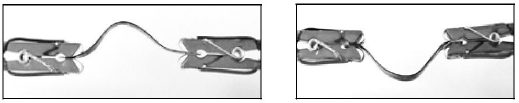
\includegraphics[width=\textwidth]{Figures/IPMC_buckle.png}
			\caption{Nafion-based IPMC in the two buckled states.}
			\label{fig:IPMC_buckle}
    \end{subfigure}

     %add desired spacing between images, e. g. ~, \quad, \qquad, \hfill etc.
      %(or a blank line to force the subfigure onto a new line)
    \begin{subfigure}[t]{0.6\textwidth}
			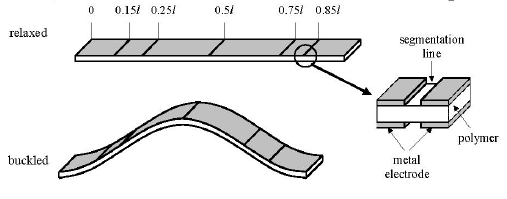
\includegraphics[width=\textwidth]{Figures/IPMC_segment.png}
			\caption{Segmentation at minimal static stress points.}
			\label{fig:IPMC_segment}
    \end{subfigure}
		\caption{Self-switching IPMC buckled beam\cite{rossiter_self-switching_2006}.}
		\label{fig:IPMC_work}
\end{figure}
For the purpose of this project, as a means of comparison, the volume of the smart required was calculated. Based on the literature of the energy density and the specifications, the volume required was calculated to be about 20 mm$^3$ for silicone and about 500 mm$^3$ for IPMCs.

\subsubsection{Magneto-strictive materials}
The magneto-strictive materials have the ability to alter their mechanical behaviour and shape when subjected to magnetic fields. Magnetic Shape Memory Alloys (MSMA) are an interesting type of magneto-strictive material. Here, the MSMA shows an interesting behaviour in which the material when deformed will tend to remain stable and retain its deformed shape. As the materials is introduced into a strong magnetic field, the crystals of the material are realigned and the material reverts back to its predeformed shape. These MSMAs are an attractive choice as they are capable of high strains around 10\% while being able to prove fast response times in the order of 1 kHz\cite{faran_ferromagnetic_2016}.

The main drawbacks of MSMAs are the fact that they are quite a new technology implying that they are expensive and that finding suppliers is quite difficult. They are also quite brittle and are thus it makes it quite difficult to find them in different geometries and shapes.

The work presented by Gauthier et al., 2006\cite{gauthier_multistable_2006} details the fabrication of a multistable actuator that is based on these MSMAs. Here the device is a push-pull actuator with a pair of agonistic-antagonistic MSMA beams. The active material is actuated using magnetic fields that are created using coils and concentrated using ferromagnetic cores. In figure \ref{fig:MSMA_princ}, a working principle of the MSMA actuator can be seen.

\begin{wrapfigure}{r}{0.45\textwidth}
	\centering
	% \vspace{20pt}
	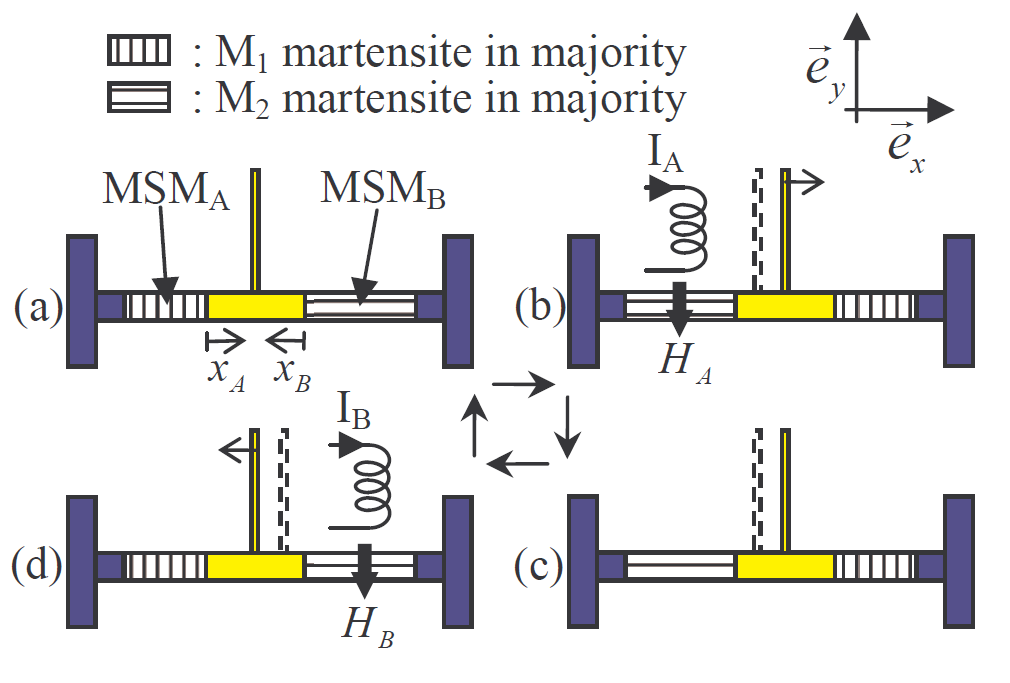
\includegraphics[width=0.4\textwidth]{Figures/MSMA_princ.png}
	\caption{Principle of the actuator\cite{gauthier_multistable_2006}.}
	% \vspace{-15pt}
	\label{fig:MSMA_princ}
\end{wrapfigure}
The shape memory effect (SME) seen in the MSMA requires the material to be deformed before the application of the magnetic field. Only after the deformation can the strain recover of the SME be observed. In this work, the team was able to create a multistable actuator by using a pair of MSMA. Here, the activation of the first MSMA deformed the opposing beam and vice versa. This results in a displacement and positioning of an end effector placed in between the MSMAs. MSMAs as with traditional SMAs have to be deformed before any actuation can be observed. This work shows the advantages and breakthrough of using an agonistic-antagonistic pair of material to resolve the problem of having to predeform the active material.

One of the important factors that leads to this technology not being widely used, is the fact that the activation of the MSMA requires magnetic fields of around 0.6 T. The work by Lu at al., 2009\cite{lu_optimal_2009} shows the relationship between strain experienced by the material and the magnetic field density. The work shows an example of a differential rotating MSMA actuator that is powered using permanent magnets and ferromagnetic cores. This study shows that the limiting factor of these technology is the activation magnetic field required for the smart material. The resulting magnetic circuits will render the fabricated actuator to be heavy and bulky. In the use case presented in this work, a rough estimation of the dimensions of the magnetic circuit was established. A basic coil system with dimensions of $23\times11\times25$ mm would be required to generate the 0.6 T needed for actuation. Thus, the MSMA material will ultimately be unsuitable for the use in small and light weight actuators as desired by this research.

\subsubsection{Shape Memory Alloys}
Shape memory alloys such NiTiNOL show two important properties: the Shape Memory Effect (SME) and Superelasticity (SE)\cite{rao_design_2015}. SMAs are a particular subgroup of smart materials that change their mechanical behaviour based on a thermal stimulus. Here, the material as with the MSMA, retains its shape when deformed and reverts back to its original shape when heated (SME). Shape Memory Alloys (SMA) actuators provide us with an opportunity to create such actuators due to their high work output per volume which is around 10 $\mathrm{J}/\mathrm{cm}^3$\cite{mohd_jani_review_2014}. This can be a 10-fold increase when compared to pneumatic actuators. The SMA actuators are thus able to provide large amounts of force when compared to their volume, making them particularly useful in compact, lightweight actuators.

SMAs are an attractive choice of material for the realisation of small and compact actuators due to their high energy density. They can provide high forces and displacements with a low volume of required material. However, they are thermally activated and have, thus, very long response times. Tomozawa et al.\cite{tomozawa_characterization_2005}, 2005, have worked on fabricating a microactuator using thin film SMA with high transformation temperatures that work at a frequency of 100Hz. The high transformation temperatures and large surface area to volume ratio allows the SMA to cool down and achieve high frequencies. Vitushinsky et al.\cite{vitushinsky_bistable_2009}, 2009 have developed also managed to create a highly responsive actuator by reducing the temperature hysteresis seen in SMAs using an actuator that is made up of two SMAs with different transition temperatures.

Paik and Wood\cite{paik_bidirectional_2012, paik_novel_2010}, 2012 devised a way to decrease the heating time of the SMAs by the way of printed-on coil. In this work, the actuator was fitted with a coil having a higher resistivity to further optimize the heating process by Joules heating. The use of an external heating element that was glued to the SMA has decreased the time response by around 30\%. Below is a simple heat exchange curve
\begin{equation}
	\label{eq:Tech}
	T(t) = (T_A - T_{\infty})e^{-t/\tau} + T_{\infty},~~\tau = \frac{C_m\rho V}{h s_{ech}}
\end{equation}
where $C_m$ is the specific heat capacity, $h$ is the heat transfer coefficient, $s_{ech}$ is the surface area of heat exchange, $V$ is the volume, $T_A$ is the austenitic finish temperature and $T_{\infty}$ is the ambient room temperature. This equation can be used to calculate the approximate time it would take to cool down the SMA material and thus determine the bandwidth of the material. Using 15 \micrometer~thick thin films or 25~\micrometer diameter thin wires and high temperature SMA (around $T_A$ = 90 \degreeC), the cooling time can be reduced to 20 ms.
A rough estimation of the required SMA for the gripper was calculated to be just around 1.5mm$^3$. Thus, a combination of the innovative ideas proposed in these above works can be used achieve effective results when designing a reactive and compact smart gripper.

\subsection{Comparison}
The aim of this section of the report is to find the most appropriate type of technology that can replace and innovate the current gripper that are employed in industry. In the current industrial era, most grippers employ the use of pneumatic actuators as their primary source of energy. Thus, to innovate the current domain of gripper, various important factors must be taken into account so as to have a point of comparison between the different smart materials and the presently used pneumatic grippers.

\begin{table}[h]
  \centering
	\footnotesize
  \caption{Comparison of actuator performances}
  \label{tab:comparison}
  \begin{tabu} to 1\textwidth {X[l, 2] X[l, 0.75] X[l,0.75] X[l,1] X[l,1] X[l,1.25]}
			\tableHeaderStyle{tableBlue}
      Actuator type & Stress [MPa] & Strain [\%] & Efficiency [\%] & Bandwidth [Hz] & Volumetric Work [J/\cc]\\
      Pneumatic \cite{mohd_jani_review_2014} & 0.7 & 50 & 90 & 20 & 0.175\\
			NiTi SMA \cite{mohd_jani_review_2014, rizzello_overview_2017, faran_ferromagnetic_2016} & 200 & 10 & 3 & $10^2$ & 10\\
			PZT \cite{kornbluh_electroelastomers:_2002, faran_ferromagnetic_2016} & 110 & 0.1 & 90 & $10^6$ & 0.1\\
			MSMA \cite{rizzello_overview_2017, faran_ferromagnetic_2016, karaca_magnetic_2009} & 100 & 6 & 90 & $10^3$ & 0.15\\
			EAP \cite{kornbluh_electroelastomers:_2002, faran_ferromagnetic_2016, rizzello_overview_2017} & 3 & 60 & 90 & $10^5$ & 0.75\\
			% Human Muscle \cite{hollerbach_comparative_1992, tadesse_electroactive_2013} & 0.8 & 100 & 35 & 173 & 0.035\\
  \end{tabu}
\end{table}
\begin{wrapfigure}{r}{0.45\textwidth}
	\centering
	\vspace{-20pt}
	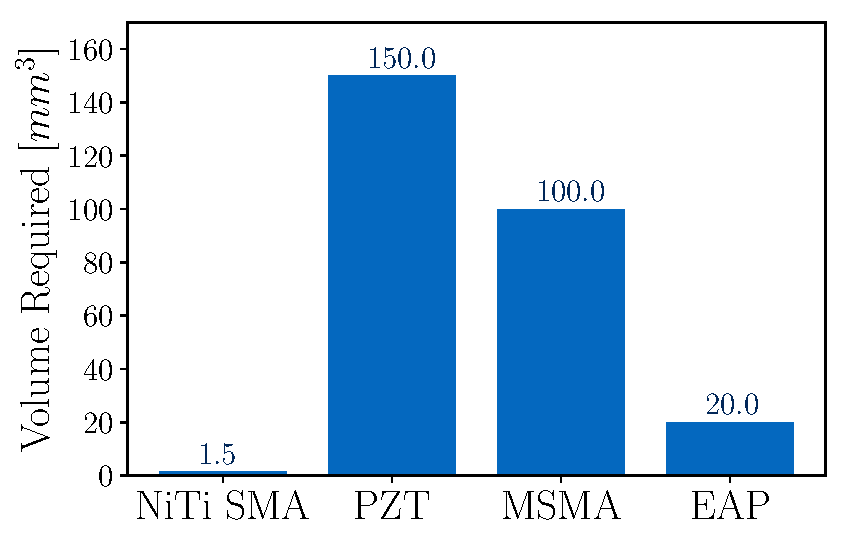
\includegraphics[width=0.4\textwidth]{Figures/Vol_Req_Bar.pdf}
	\vspace{-5pt}
	\caption{Approximate volume of the smart material required for the gripper based on the specifications and the volumetric work.}
	% \vspace{-5pt}
	\label{fig:vol_req_bar}
\end{wrapfigure}
In the hopes of creating a compact and lightweight actuator, the most important parameter to consider would be the volumetric work. This parameters determines the level at which the active component of the actuator can be minimised when designing the gripper. The SMA offers a great deal better work output to volume ratio when compared to the other materials. The most critical aspect in this case would be attempting to optimize the time response of these SMA in hopes of improving a critical parameter in which this material is lacking.


% \begin{figure}[H]
% 	\centering
% 	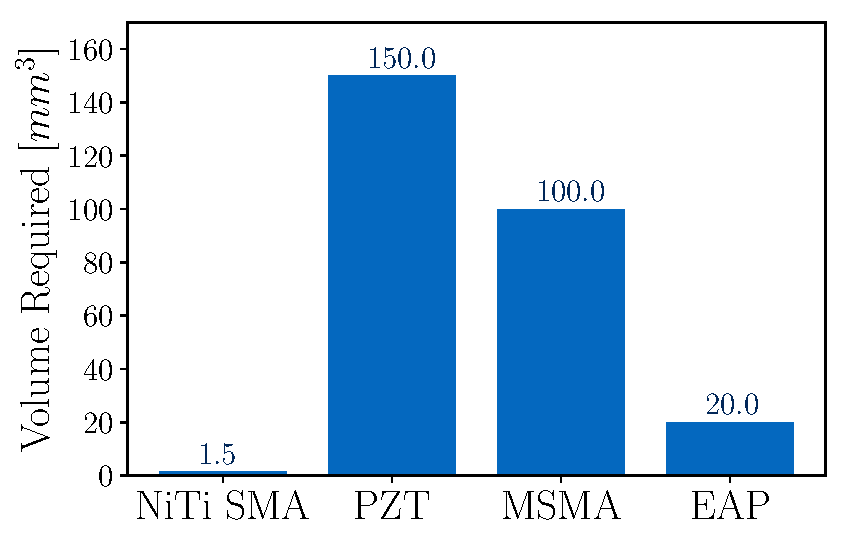
\includegraphics[width=0.4\textwidth]{Figures/Vol_Req_Bar.pdf}
% 	\caption{Approximate volume of the smart material required for the gripper based on the specifications and the volumetric work.}
% 	\label{fig:vol_req_bar}
% \end{figure}
